\documentclass{article}


\usepackage{amsmath}
\usepackage{amssymb}
\usepackage{graphicx}
\usepackage{color}
\usepackage{subfig}
\usepackage{float} % For [H] placement

\usepackage[ruled,vlined,linesnumbered]{algorithm2e}

\usepackage{booktabs}

\usepackage[bookmarks=true,ocgcolorlinks=true,plainpages=false, breaklinks=true, bookmarksopen=true, bookmarksnumbered=true]{hyperref}
%\hypersetup{bookmarks=false}  %hide the bookmarks bar
%\hypersetup{bookmarksopen=false}  % expand tree of bookmarks or just show first level
\hypersetup{linkcolor=blue, citecolor=magenta,urlcolor=blue} % electronic
\hypersetup{colorlinks=true}

\usepackage[T1]{fontenc}
\usepackage{palatino}

\allowdisplaybreaks

\renewcommand{\vec}[1]{\ensuremath{{\boldsymbol #1}}}
\newcommand{\mat}[1]{\ensuremath{\boldsymbol{#1}}}


\title{Statistical performance analysis of neural mass models?}
\date{\today}

\begin{document}


\section{Introduction}


History of models and estimation attempts

Usefulness of bound: benchmark algorithms, experimental design, insight about inherent uncertainty -- which do we address


Not claiming anything about which model is the 'best', but simply what level of complexity is possible - how increasing complexity affects uncertainty.
\section{Background}



\paragraph{Neural Mass Model}
\begin{figure}[ht]
  \begin{center}
    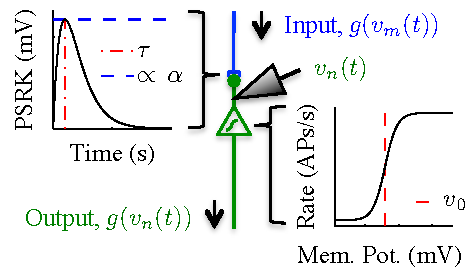
\includegraphics{./figures/pdf/SingleMass.pdf}
  \end{center}
  \caption{\emph{\textbf{Neural Mass Model.} The somas of the neural mass are represented by the triangle. The synaptic connections are represented by the circle. The input mean firing rate, $g(v_m(t))$, is convolved with post-synaptic response kernel (PSRK), shown in the inset on the left, to give the mean membrane potential, $v_n(t)$. This is transformed by the sigmoid, shown in the inset on the right, to give the output mean firing rate, $g(v_n(t))$.}}
  \label{fig:SingleNeuralMass}
\end{figure}
Neural mass models map from a mean firing rate of a population of pre-synaptic neurons to a mean membrane potential of a post-synaptic population, which in turn determines that population's output firing rate. A graphical description of a neural mass model can be seen in Figure~\ref{fig:SingleNeuralMass}. 

To define a standard neural mass model, we begin by defining the post-synaptic potential of population $n$, $v_n(t)$, as a result of an input firing rate from population $m$, $g(v_m(t))$, as the convolution
\begin{equation}\label{eq:conv_eq}
    v_n(t) = \frac{\alpha_{mn}}{\tau_{mn}}\int_{-\infty}^t  h_{mn}(t-t')g(v_m(t')) \,\mathrm{d}t',
\end{equation}
where $\alpha_{mn}$ is the gain for the post-synaptic response kernel (PSRK), denoted by $h_{mn}(t)$, from neural population $m$ to $n$, and $\tau_{mn}$ is the membrane time constant. A common form of the PSRK is
\begin{equation}
    h_{mn}(t) = \eta(t)t\exp\left(-\frac{t}{\tau_{mn}}\right),
\end{equation}
where $\eta(t)$ is the Heaviside step function. An example of a PSRK can be seen in the left inset of Figure~\ref{fig:SingleNeuralMass}.  

The firing rate of each population is related to the mean membrane potential by a sigmoidal activation function; the logistic function sigmoid is typically used: 
\begin{align}
    g\left(v_n(t)\right) =& \frac{1}{1+\exp{\left(\varsigma_n\left(v_{0n} - v_n(t)\right)\right)}}.
    \label{eq:sigmoid}
\end{align}
The quantity $\varsigma_n$ describes the slope of the sigmoid (approximating the variance of firing thresholds within the populations) and $v_{0n}$ describes the mean firing threshold. An example of the sigmoidal activation function can be seen in the right inset of Figure~\ref{fig:SingleNeuralMass}.

The convolution in Equation~\ref{eq:conv_eq} can also be written as the ordinary differential equation (ODE)
\begin{equation}\label{eq:2ndOrder}
    \mathrm{D}v_n(t) = \frac{\mathrm{d}^2 v_n(t)}{\mathrm{d}t^2} + \frac{2}{\tau_{mn}}\frac{\mathrm{d} v_n(t)}{\mathrm{d}t} + \frac{1}{\tau_{mn}^2} v_n(t) = \frac{\alpha_{mn}}{\tau_{mn}} g(v_m(t)),
\end{equation}
where $\mathrm{D}$ is a linear differential operator. Equation~\ref{eq:2ndOrder} can be written as two coupled first-order ODEs by 
\begin{equation} \label{eq:2ndOrderNMM}
    \frac{\mathrm{d} v_n(t)}{\mathrm{d}t} = z_n(t),\,\,\,\,\,    \frac{\mathrm{d}z_n(t)}{\mathrm{d}t} = \frac{\alpha_{mn}}{\tau_{mn}} g(v_m(t)) - \frac{2}{\tau_{mn}}z_n(t) - \frac{1}{\tau_{mn}^2} v_n(t),
\end{equation}
where $z_n(t)$ is a dummy variable. This forms the basis of a state-space model in a canonical format.

The parameters of the model, $\tau$, $\alpha$, $v_0$ and $\varsigma$, can be set so the neural mass has characteristics of specific neural populations, such as pyramidal neurons, spiny stellate cells and fast and slow inhibitory interneurons (GABA$_\mathrm{a}$ and GABA$_\mathrm{b}$). The neural populations can then be connected to represent the circuitry of a cortical column and further to form networks of columns. Various kinds of neural mass models have been developed \cite{Silva1974,Jansen1995,Wendling2002,David2003}, which are depicted in Figure~\ref{fig:NMMs}. Each synaptic connection in these networks can be described by the 2$^{\mathrm{nd}}$-order system of Equation~\ref{eq:2ndOrderNMM}, where the resultant dimensions of the networks of neural mass models in Figures~\ref{fig:NMMs} a, b and c are 6, 12 and 18, respectively.
\begin{figure}[ht]
	\centering
		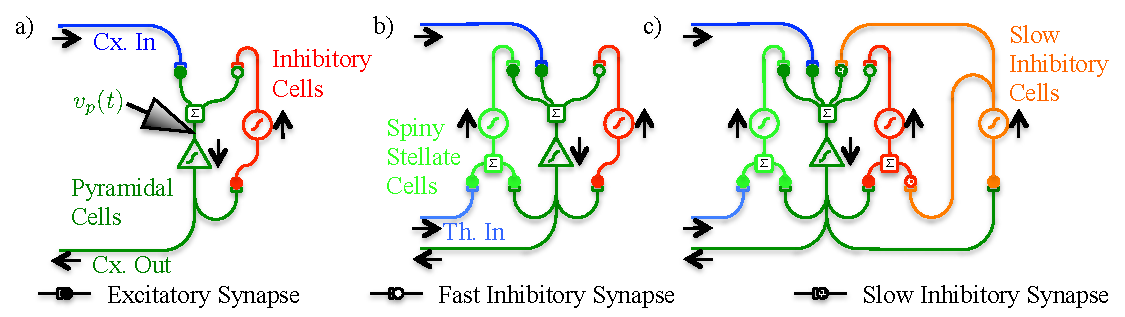
\includegraphics[scale=1]{./figures/pdf/NeuralMassesHoriz.pdf}
	\caption{\emph{\textbf{Models of Cortical Columns.} Each model has a pyramidal neural population, with various forms of feedback and inputs (Cx. = Cortex, Th. = Thalamus). The EEG is taken as the mean membrane potential of the pyramidal population, $v_p(t)$, with additive measurement noise.  a) Minimal model of a column with inhibitory feedback \cite{Silva1974}. b) An extension with excitatory feedback and afferent input from thalamus \cite{Jansen1995,David2003}. c) Column with inhibition occurring across two times scales, enabling modelling of higher frequency activity observed in seizures~\cite{Wendling2002}.}}
	\label{fig:NMMs}
\end{figure}

\begin{figure}[ht]
	\centering
		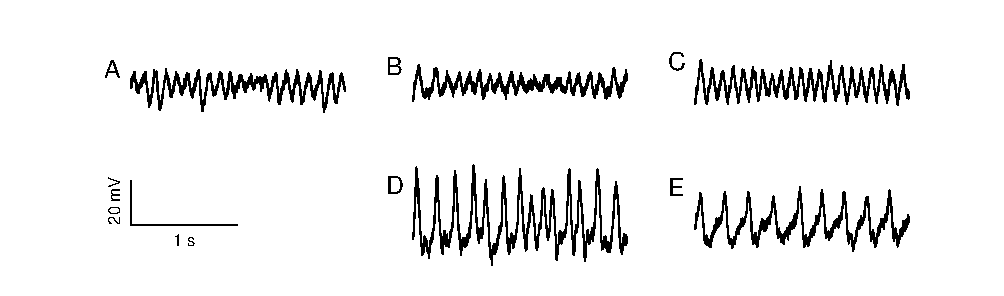
\includegraphics[scale=1]{./figures/pdf/Example_Data.pdf}
		\caption{\textbf{Example data generated using the neural mass models.}}
	\label{fig:NMMs}
\end{figure}


The parameters of the neural masses not only define the population type, but also the behaviour exhibited by the model. For example, certain parameter combinations result in a model of a cortical column that will generate alpha wave type activity (normal activity) and, for another set of parameters, we create a model that will exhibit epileptic behaviour \cite{Wendling2002}. Therefore, we consider a family of models, which we define generally as 
\begin{align}\label{eq:NeuralMassModel}
    \dot{\mathbf{x}}(t) =& f_{\theta}\left(\mathbf{x}(t),\mathbf{u}(t)\right)\\
    y(t) =& \mathbf{C}\mathbf{x}(t) + e(t),
\end{align}
where $\mathbf{x}(t) \in \mathbb{R}^{n_x}$ is a state vector representing the postsynaptic membrane potentials generated by each population synapse and their time derivatives, $n_x$ is the number of states and $\mathbf{u}(t)$ represents the system input, which may be from afferent connections or other brain regions, exogenous input, or account for model inaccuracies. The function $f_{\theta}(\cdot)$ describes the dynamics, where $\theta \in \mathbb{R}^{n_{\theta}}$ determines the model type and the behaviour it exhibits. The iEEG is denoted by $y(t)$, $\mathbf{C}$ is the observation matrix, and $e(t)$ is the observation noise.

The model focused on in the following
estimation sections is the formulation by Jansen and Rit \cite{Jansen-Rit-95}.
Given space limitations we refer the reader to the article by Jansen
and Rit\cite{Jansen-Rit-95} where the original state-space equations
are presented. The parameters that were described in this section are related to the Jansen and Rit paper by
\begin{align}
    A =& \frac{\alpha_{pe}}{2e_0c_1} = \frac{\alpha_{pi}}{2e_0c_3} = \frac{\alpha_{ep}}{2e_0c_2} = \frac{\alpha_{xp}}{2e_0} \\
    B =& \frac{\alpha_{ip}}{2e_0c_4} \\
    a =& \frac{1}{\tau_{pe}} = \frac{1}{\tau_{pi}} = \frac{1}{\tau_{ep}} = \frac{1}{\tau_{xp}} \\
    b =& \frac{1}{\tau_{ip}},
\end{align}
where $e_0$ is a parameter that scales the maximum firing rate, $A$ and $B$ are synaptic gains for excitation and inhibition respectively, and $a$ and $b$ are the reciprocals of the synaptic time constants for excitation and inhibition, respectively, and the subscripts $p$, $e$, $x$, and $i$ denote pyramidal ($p$), excitatory interneuron (spiny stellate) ($e$), external ($x$) or inhibitory interneuron ($i$) populations, respectively. By making the assumption that all excitatory synapses share the same time constants and by defining the connectivity constants, $c_1$, $c_2$, $c_3$ and $c_4$, the network of neural masses is the JR NMM.

Present 3 models?

\section{Theory / Performance Bounds}

Introduce recursive computation of bound and Monte Carlo approximation

\section{Methods?}

\section{Results}

\subsection{Effect of increasing model complexity -- bound should increase}

e.g. Bound for model A > model B > model C

\subsection{Effect of parameters changing -- bound should change}

e.g. seizure easier to estimate than alpha rhythms

\subsection{Effect of measurement noise? -- pretty boring}

e.g. scalp EEG vs iEEG?

\subsection{Augmented models (joint estimation of parameters and states)?}

\section{Discussion}

extensions to other applications e.g. experimental design

contextualize work w.r.t. existing literature?

\section{Conclusion}


\small
\bibliographystyle{ieeetr}
\bibliography{References}




\end{document}
